\section{结果}
\label{sec:results}

\subsection{增加病例量对平均再生数估计的收益递减}
\label{sec:res-theory}

\begin{figure}[t]
  \centering
  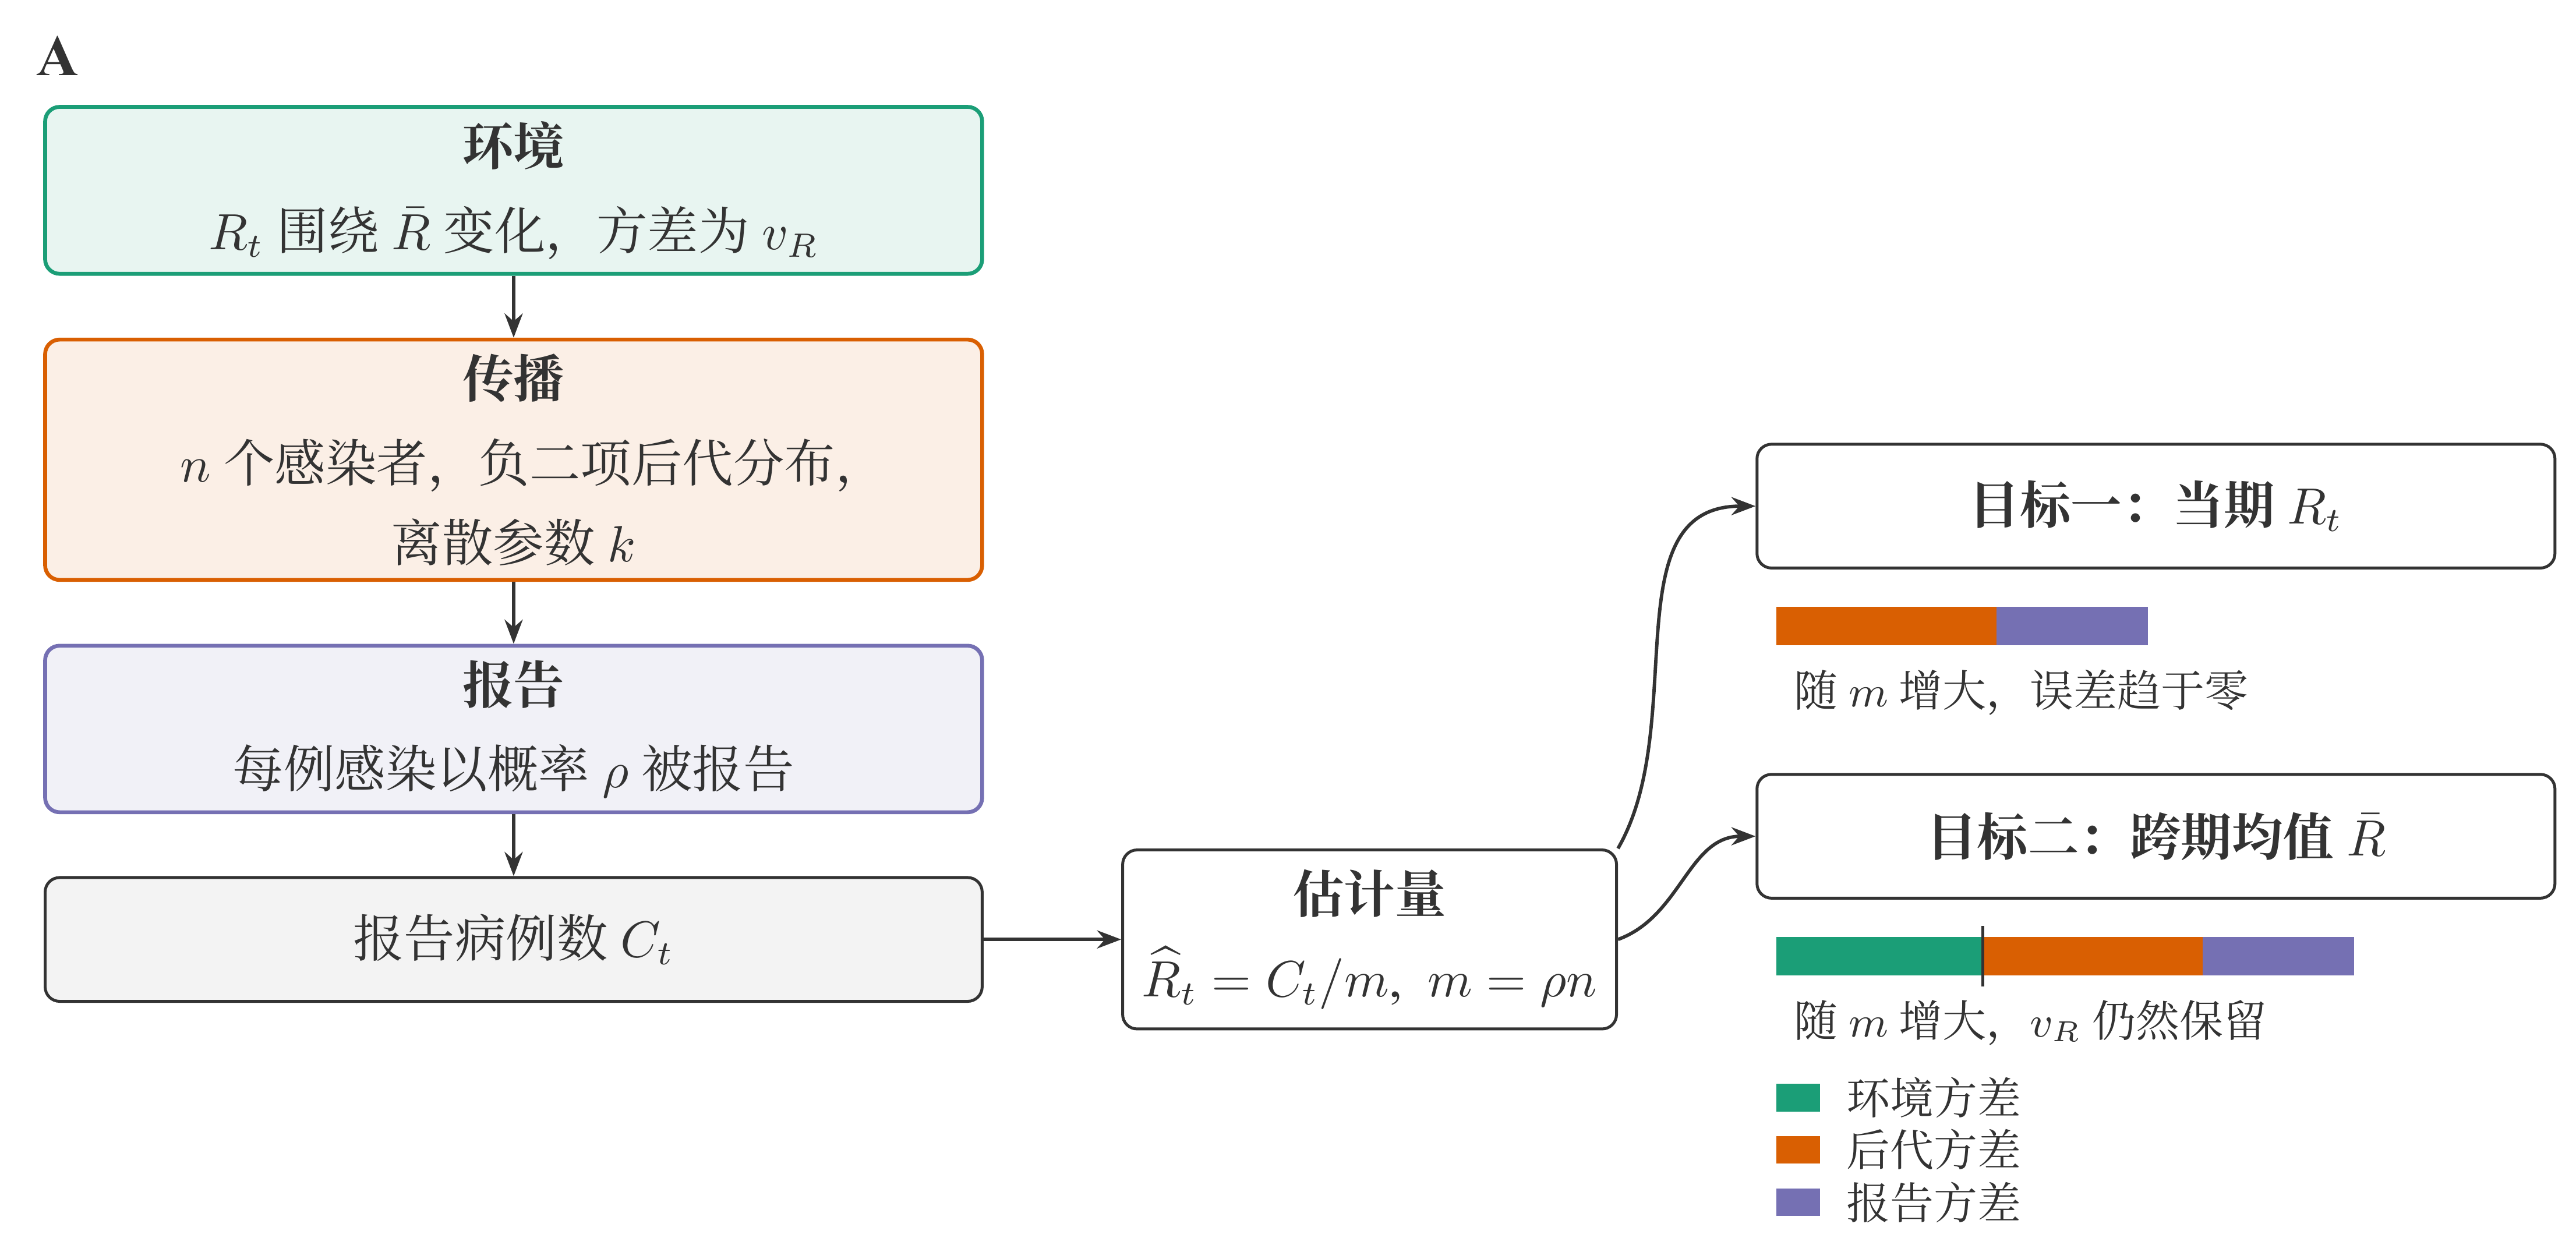
\includegraphics[width=0.86\linewidth]{figures/fig_01_schematic.png}\\[2pt]
  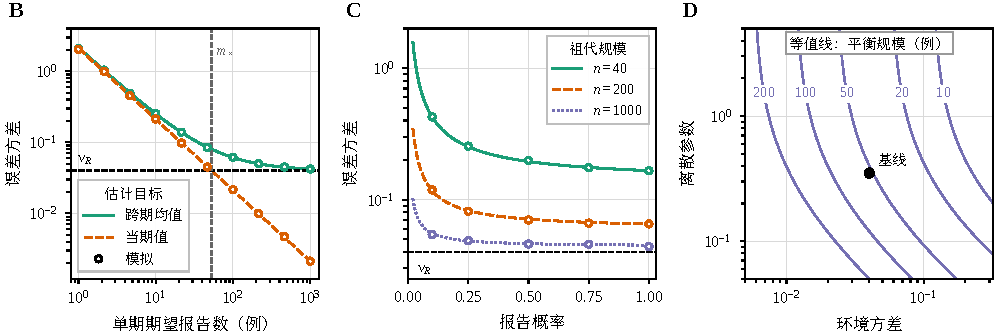
\includegraphics[width=\linewidth]{figures/fig_01_theory.pdf}
  \caption{环境变异、后代变异与报告变异对再生数尺度化估计量误差的贡献。（A）以报告病例数除以期望病例量的估计量及其两个估计目标（当期值与跨期均值）的示意图，颜色区分环境、后代与报告三类误差来源。（B）固定报告概率时，跨期均值与当期值的误差方差随单期期望报告病例数的变化；曲线为闭式解，圆点为蒙特卡罗估计及其 95\% 区间，虚线标出环境方差 $v_R$ 与平衡规模。（C）三种固定原发病例数下误差方差随报告概率的变化；完全报告时的取值为残余后代项。（D）平衡规模在环境方差与后代离散参数平面上的等值线，图中标出基线参数组合。}
  \label{fig:theory}
\end{figure}

在基线参数下（$\Rbar=1.15$，$v_R=0.04$，$k=0.35$，$\rho=0.25$），抽样系数 $A=2.1232$，平衡规模为每期 $\mx=53.1$ 例报告病例（图~\ref{fig:theory}B）。当期值的误差方差在整个范围内与 $1/m$ 成比例下降，跨期均值的误差方差则逐渐趋于 $v_R$。固定 $\rho$ 而经由覆盖规模使病例量加倍时，跨期均值的误差方差在 $m=10$ 处下降 42.1\%，在 $m=\mx$ 处下降 25.0\%，在 $m=200$ 处下降 10.5\%。每个点基于 20000 次重复的蒙特卡罗估计与式~(\ref{eq:var-average}) 的偏差至多为 4.0\%。

固定覆盖规模而提高报告概率，误差方差始终高于 $v_R$ 的水平（图~\ref{fig:theory}C）。完全报告时，原发病例数为 40、200 和 1000 的残余方差分别为 0.166、0.0652 和 0.0450。以基线下位于平衡规模的覆盖规模 $n=212.3$ 为例，报告概率由 0.25 提高到 0.50 只使误差方差下降 13.5\%，而经由 $n$ 使病例量加倍可下降 25.0\%；即使完全报告，误差方差仍为 0.0638。在基线附近，覆盖规模按某一比例增加时误差方差的降幅，是报告概率按相同比例增加时降幅的 $A/\Rbar=1.85$ 倍。环境方差较小且后代分布高度过离散时，平衡规模最大（图~\ref{fig:theory}D）。

\begin{figure}[t]
  \centering
  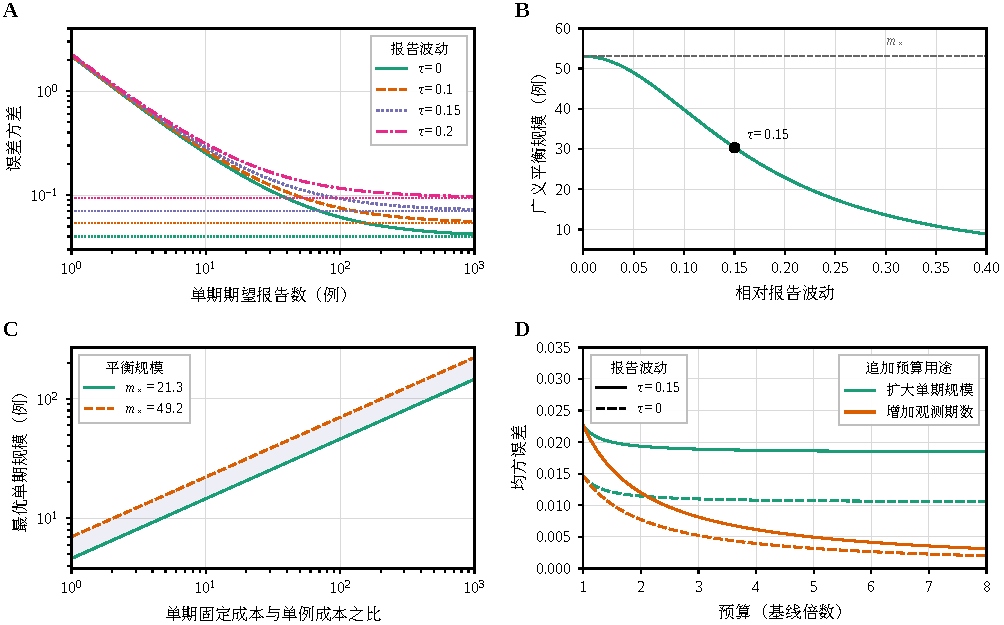
\includegraphics[width=0.92\linewidth]{figures/fig_02_heterogeneity_budget.pdf}
  \caption{报告异质性与固定监测预算的分配。（A）四种相对报告波动水平下误差方差随单期期望报告病例数的变化；点线为病例量增大时相应的极限值，由环境方差与报告方差之和决定。（B）广义平衡规模随相对报告波动的变化；虚线为无报告波动时的平衡规模，圆点为面板（D）所用的波动水平。（C）取平衡规模情景范围的两端时，单期最优报告病例数随价格比 $c_0/c_1$ 的变化；阴影带覆盖两端之间的范围。（D）环境变异与报告变异均存在自相关时，平均再生数估计量的均方误差随总预算的变化，追加预算分别用于增加单期病例数或增加时期数；实线为基线报告，虚线为标准化报告。}
  \label{fig:budget}
\end{figure}

相对报告波动 $\tau=0.15$ 使极限方差增加 $v_H=0.0307$，并使平衡规模由 53.1 例降至 30.4 例（图~\ref{fig:budget}A、B）。按流感住院设定的情景参数，潜在平衡规模为 21.3--49.2 例。在此范围内，式~(\ref{eq:optimal-m}) 给出的最优病例量 $m^*$ 在 $c_0/c_1=10$ 时为每期 14.6--22.2 例，在 $c_0/c_1=100$ 时为每期 46.2--70.1 例（图~\ref{fig:budget}C）；在基线 $\mx=53.1$ 下分别为 23.0 例与 72.9 例。若固定 $n=212.3$ 而以报告概率为决策变量，$c_0=100$、$c_\rho=c_1n$ 时的最优报告概率为 $\rho^*=0.209$。在一个假设示例中，设共有十期、每期 50 例，环境与报告均存在自相关（$\phi=\psi=0.5$），且 $\tau=0.15$，此时跨期均值的均方误差为 $22.57\times10^{-3}$，其中环境部分为 $10.40\times10^{-3}$，报告部分为 $7.88\times10^{-3}$，抽样部分为 $4.29\times10^{-3}$（表~\ref{tab:s7}）。病例量增至十倍时，均方误差降至 $18.71\times10^{-3}$；报告标准化使其降至 $14.65\times10^{-3}$，时期数增至四倍则使其降至 $6.17\times10^{-3}$。预算为基线的两倍时，将增量用于病例所得均方误差为 $19.35\times10^{-3}$，用于时期所得均方误差为 $11.98\times10^{-3}$（图~\ref{fig:budget}D）。

\subsection{流感住院数据中的截距与表观平衡规模}
\label{sec:res-empirical}

\begin{figure}[t]
  \centering
  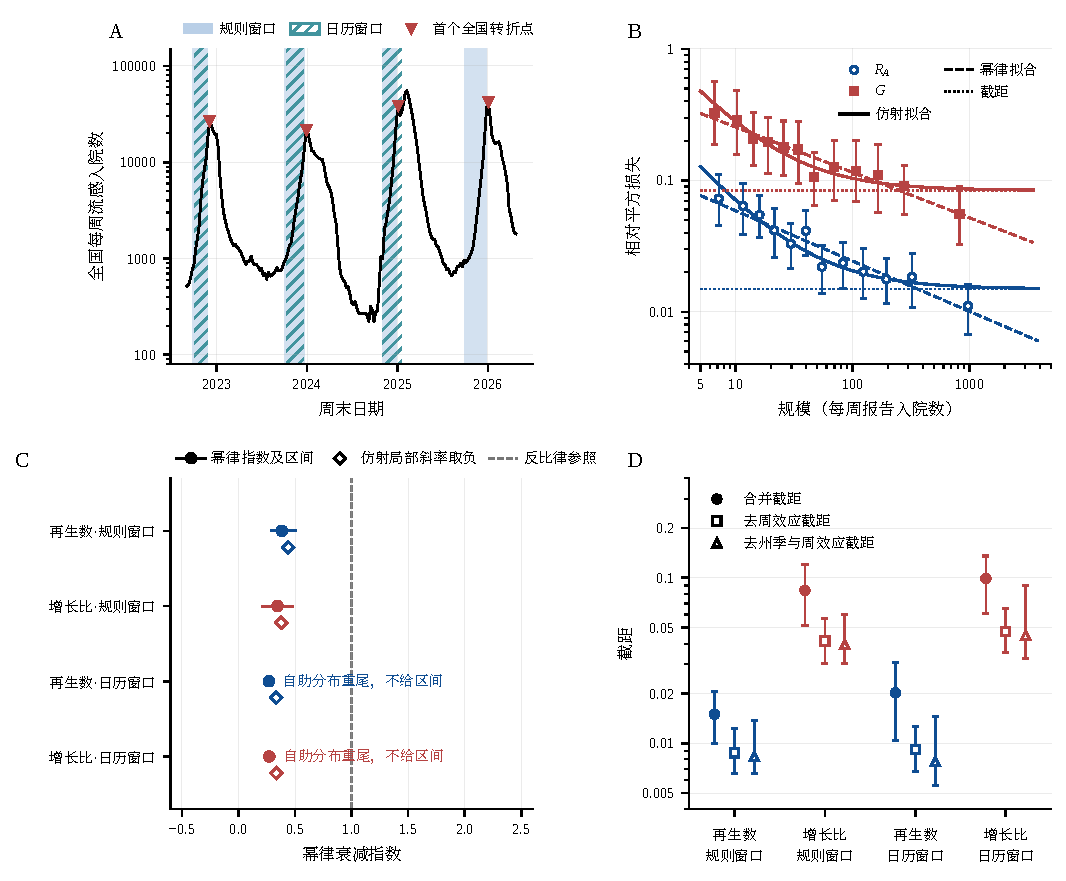
\includegraphics[width=\linewidth]{figures/fig_03_empirical_loss.pdf}
  \caption{流感住院数据中两种周增长统计量的相对损失。（A）对数尺度下的全国每周流感住院人数；浅蓝阴影为规则窗口（$S=4$），斜线为日历窗口（$S=3$），三角形标出各流行季的首个全国转折点。（B）规则窗口中两种统计量按规模变量 $M$ 固定分为 12 个分箱的平均相对损失，误差线为州 $\times$ 周双向自助 95\% 百分位区间；实线为仿射拟合 $a+b/M$，虚线为无截距幂律拟合 $cM^{-\gamma}$，点线为截距 $a$。（C）幂律指数 $\gamma$ 的点估计，规则窗口附双向自助 95\% 百分位区间，日历窗口仅给点估计；空心菱形为仿射拟合在样本规模处局部对数斜率均值的相反数；虚线为 $\gamma=1$ 参照。（D）四种设定下的截距、去除全国周效应后的截距以及同时去除周效应与州--季效应后的截距，误差线为双向自助 95\% 百分位区间。}
  \label{fig:floor}
\end{figure}

在四个流行季的规则窗口中，42 个日历周内的 1748 个州周给出更新型比值的截距 $a=0.0150$（95\% CI：0.0100, 0.0205）、斜率 $b=0.560$（95\% CI：0.375, 0.761）以及表观平衡规模 $b/a=37.4$（95\% CI：19.7, 69.7；图~\ref{fig:floor}B，表~\ref{tab:s1}）。同一窗口中，加权增长比由 1756 个州周给出 $a=0.0840$（95\% CI：0.0515, 0.1199）和 $b/a=23.5$（95\% CI：8.8, 54.7）。两种统计量的样本差异来自规模条件，有 8 个州周的 $D_t\ge5$ 而当周住院数少于 5。三个日历窗口中，$R_A$ 给出 $a=0.0202$（95\% CI：0.0104, 0.0307）与 $b/a=25.6$（95\% CI：10.1, 73.9），$G$ 给出 $a=0.0991$（95\% CI：0.0608, 0.1356）与 $b/a=22.6$（95\% CI：9.4, 48.9）。四种设定的截距区间都位于零以上。截距的双向自助标准差是仅对州重抽样所得标准差的 1.96--3.49 倍；仅对州重抽样时，规则窗口 $R_A$ 截距的区间为 0.0124--0.0178，明显窄于双向区间。

在观测到的规模范围内，无截距幂律对分箱损失的拟合与仿射形式接近（图~\ref{fig:floor}B）。规则窗口中幂律指数 $\gamma$ 对 $R_A$ 为 0.38（95\% CI：0.29, 0.51），对 $G$ 为 0.35（95\% CI：0.21, 0.48）；仿射拟合在样本规模处的平均局部对数斜率分别为 $-0.44$ 与 $-0.38$（图~\ref{fig:floor}C，表~\ref{tab:s2}）。两组数值都远离反比律对应的 $-1$，说明在这一规模范围内损失随规模下降得比纯计数噪声慢。日历窗口的幂律指数点估计均为 0.27。$\gamma$ 与平均局部斜率出自不同的拟合目标，二者的接近只是几何上的对应。仿射形式的参数与命题~\ref{prop:average} 一一对应，因此后续分析以仿射形式为准。

\subsection{截距的多尺度分解}
\label{sec:res-multiscale}

截距包含同一日历周内各州共有的分量和各州特有的分量（图~\ref{fig:floor}D；表~\ref{tab:s2}）。去除全国周效应后，规则窗口中 $R_A$ 的截距由 0.0150 降至 0.0088（95\% CI：0.0066, 0.0122），全国周份额为 41\%（95\% CI：12, 57）；$G$ 的截距由 0.0840 降至 0.0415（95\% CI：0.0304, 0.0569），份额为 51\%（95\% CI：21, 65）。日历窗口中这一份额对 $R_A$ 为 55\%，对 $G$ 为 52\%。再去除州--季效应后截距变化很小，规则窗口中 $R_A$ 降至 0.0083（95\% CI：0.0066, 0.0137），$G$ 降至 0.0394（95\% CI：0.0305, 0.0602），四种设定中州--季分量的区间均包含零。同一周内的共有分量在统计上是全国周效应，不对应某个可单独识别的传播或报告机制。

全国周分量在同一周内进入每个州的损失。某州住院数增加只能缩小该州的计数项，对多州取平均只能缩小州特有项，两者都消除不了共有分量，只有增加观测周数才能把它平均掉。按式~(\ref{eq:pooling}) 的形式，若各州残差独立且规模相近，$J$ 个州合并后的截距约为单州的 $w+(1-w)/J$，其中 $w$ 为全国周份额；$R_A$ 在 $J=5$、10 和 51 时约为单州的 0.53、0.47 和 0.42，$G$ 约为 0.61、0.56 和 0.51（图~\ref{fig:design}C）。

\subsection{报告完整度}
\label{sec:res-reporting}

\begin{figure}[t]
  \centering
  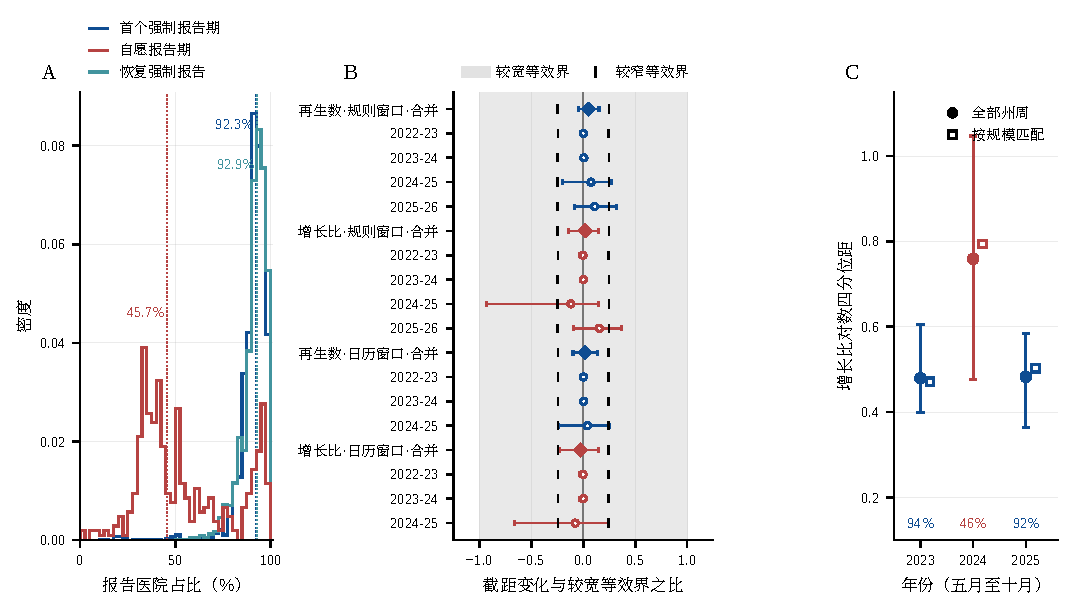
\includegraphics[width=0.86\linewidth]{figures/fig_04_reporting.pdf}
  \caption{报告完整度与截距。（A）报告规模不低于 5 的州周中报告医院占比在三个报告期的分布，点线为中位数。（B）规则窗口与日历窗口中覆盖调整前后截距之差 $\Delta a$，以 $\tau_0=0.10$ 的等效界为单位。菱形为合并估计，圆圈为分季估计，误差线为配对双向自助 90\% 百分位区间。灰带与竖刻线分别为 $\tau_0=0.10$ 与 $\tau_0=0.05$ 的等效界。（C）各年 5 月至 10 月 $\log G$ 的四分位距及州 $\times$ 周双向自助 95\% 百分位区间，空心方块为按报告规模匹配后的值，底部数字为报告医院占比中位数。}
  \label{fig:reporting}
\end{figure}

在报告规模不低于 5 的州周中，报告医院占比的中位数在第一个强制报告期为 92.3\%，在自愿报告期为 45.7\%，恢复强制报告后为 92.9\%（图~\ref{fig:reporting}A）。规则窗口内的中位数为 93.7\%，79.8\% 的州周至少有 90\% 的医院报告。在这些窗口中，按报告占比调整统计量后，$R_A$ 的截距变化 $\Delta a=0.29\times10^{-3}$（90\% CI：$-0.24\times10^{-3}$, $0.83\times10^{-3}$），$G$ 的截距变化为 $0.37\times10^{-3}$（90\% CI：$-2.76\times10^{-3}$, $2.95\times10^{-3}$）（图~\ref{fig:reporting}B；表~\ref{tab:s3}）。相对波动 $\tau_0=0.10$ 的独立报告冲击使 $R_A$ 与 $G$ 的截距平均增加 $5.45\times10^{-3}$ 与 $20.09\times10^{-3}$，约为各自截距的 36\% 与 24\%；$\tau_0=0.05$ 时为 $1.35\times10^{-3}$ 与 $4.95\times10^{-3}$，约为截距的 9\% 与 6\%。两项变化在两个等效界下均判为等效，日历窗口的结果相同。分季检验中，$\tau_0=0.10$ 时全部流行季等效，$\tau_0=0.05$ 时规则窗口四季中有两季、日历窗口三季中有两季等效。在强制报告期内，机构报告参与度的变化对截距的影响因此小于相对波动 5\% 的独立报告冲击所产生的影响。

报告完整度明显偏低的对照只有自愿报告期这一段。5 月至 10 月期间，$\log G$ 的四分位距在自愿报告的 2024 年为 0.76，在 2023 年与 2025 年均为 0.48（图~\ref{fig:reporting}C；表~\ref{tab:s4}）。2024 年与 2023 年之比为 1.58（95\% CI：0.95, 2.23），与 2025 年之比为 1.57（95\% CI：0.95, 2.39），作为对照的 2025 年与 2023 年之比为 1.01（95\% CI：0.72, 1.25）。三年同期的报告规模中位数相近（15.6、16.6 和 16.2 例），按报告规模分布重新加权后，两个比值为 1.68 和 1.58。按日历月匹配时，十二组月份--年份比较中有九组大于 1，比值中位数为 1.33。自愿报告期的离散度因此在点估计上约高出六成，但两个比值的 95\% 区间均包含 1。

\subsection{收益递减与监测设计}
\label{sec:res-design}

\begin{figure}[t]
  \centering
  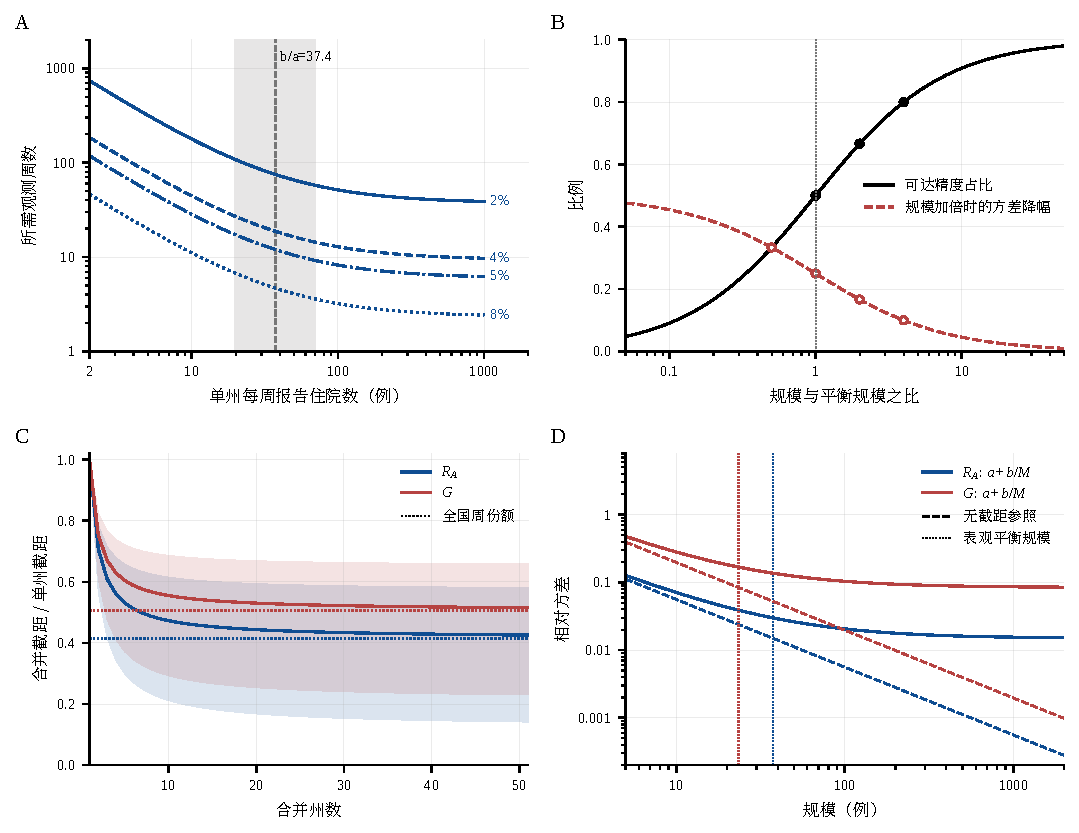
\includegraphics[width=\linewidth]{figures/fig_05_design_nomogram.pdf}
  \caption{监测设计列线图。（A）单州平均更新型比值的相对标准误达到 2\%、4\%、5\% 与 8\% 所需的观测周数 $T=(a+b/M)/s^2$，按规则窗口 $R_A$ 的拟合值计算并假定周间独立；虚线为表观平衡规模 $b/a$，灰带为其双向自助 95\% 区间。（B）以平衡规模为单位时，可达精度占比 $(m/\mx)/(1+m/\mx)$ 与规模加倍时的相对方差降幅 $1/[2(1+m/\mx)]$，圆点标出 $m/\mx=0.5$、1、2、4。（C）由全国周份额 $w$ 推算的 $J$ 州合并截距与单州截距之比 $w+(1-w)/J$，阴影由 $w$ 的 95\% 区间端点给出，点线为 $w$。（D）两种统计量的拟合相对方差 $a+b/M$ 与无截距参照 $b/M$，点线为各自的表观平衡规模。}
  \label{fig:design}
\end{figure}

在 $V(m)=a+b/m$ 下，病例量不受限时可达精度中能够实现的份额为 $m/(m+\mx)$，$m$ 加倍一次使方差降低 $\mx/[2(m+\mx)]$（命题~\ref{prop:average}）。$m$ 为 $\mx$ 的 0.5、1、2 和 4 倍时，这一份额依次为 33\%、50\%、67\% 和 80\%，由这些位置再加倍一次，方差依次下降 33\%、25\%、17\% 和 10\%；要实现可达精度的 90\%，需要 $m=9\mx$（图~\ref{fig:design}B）。以表观平衡规模代入，规则窗口中 $R_A$ 有 55\%、$G$ 有 65\% 的州周位于 $b/a$ 之上，分别有 25\% 与 32\% 位于 $4b/a$ 之上。对单个州而言，使平均 $R_A$ 达到给定相对标准误所需的观测周数在住院数低于 $b/a$ 时随住院数增加而迅速减少，高于约 $4b/a$ 后几乎不再变化（图~\ref{fig:design}A）。以表观平衡规模和成本比 $c_0/c_1=10$ 代入式~(\ref{eq:optimal-m})，$R_A$ 尺度上的最优病例量为 $m^*=19.4$（95\% CI：14.0, 26.4），$G$ 为 15.3；$c_0/c_1=100$ 时为 61.2 和 48.4。

不含截距的计数噪声模型给出的相对方差为 $b/M$（图~\ref{fig:design}D）。拟合方差与之之比为 $1+M/(b/a)$，在 $M=b/a$ 时为两倍，在 $M=9\,b/a$ 时为十倍；对 $R_A$ 而言，相应位置为每周 37 例与 337 例住院。在多数州周所处的规模上，只按计数噪声计算的不确定性因此明显偏窄。

\subsection{流行季间异质性与分母权重}
\label{sec:res-seasons}

流行季数量限制了对季间变异的估计（图~\ref{fig:seasons}；表~\ref{tab:s5}）。规则窗口中 $R_A$ 的分季截距依次为 0.0137、0.0062、0.0127 和 0.0225，随机效应合并截距为 0.0123（95\% CI：0.0021, 0.0225），$I^2=0.53$。$G$ 的合并截距在规则窗口中为 0.0610（95\% CI：$-0.0010$, 0.1231），在日历窗口中为 0.0745（95\% CI：$-0.0697$, 0.2186）；只有三到四个流行季时，$t_{S-1}$ 区间很宽。季间方差的任何无偏估计，其相对标准误在三个流行季时至少为 1.00，四个流行季时至少为 0.82（推论~\ref{cor:season}）。

规则窗口中，以单周计数为分母时 $G$ 的截距为原权重时的 $q_1=0.660$（95\% CI：0.562, 0.792），以等权三周为分母时为 $q_2=1.597$（95\% CI：1.384, 1.845）（表~\ref{tab:s6}）。只含报告噪声与平滑流行曲线的零模型同样产生 $q_1<1<q_2$ 的排序，其比值均值的范围为 $q_1$ 0.760--1.067、$q_2$ 1.055--1.464；观测点估计位于两个范围之外，但落在范围之外的双侧 $p$ 值为 0.120 与 0.217。要求各季窗口不少于四周时，零模型范围为 0.762--1.077 与 1.051--1.462。比值的排序本身因此不足以区分环境变异与报告噪声；分母报告噪声改变截距的机制见附录~\ref{app:random-denominator}。

\subsection{潜在环境方差的模拟反演}
\label{sec:res-inversion}

\begin{figure}[t]
  \centering
  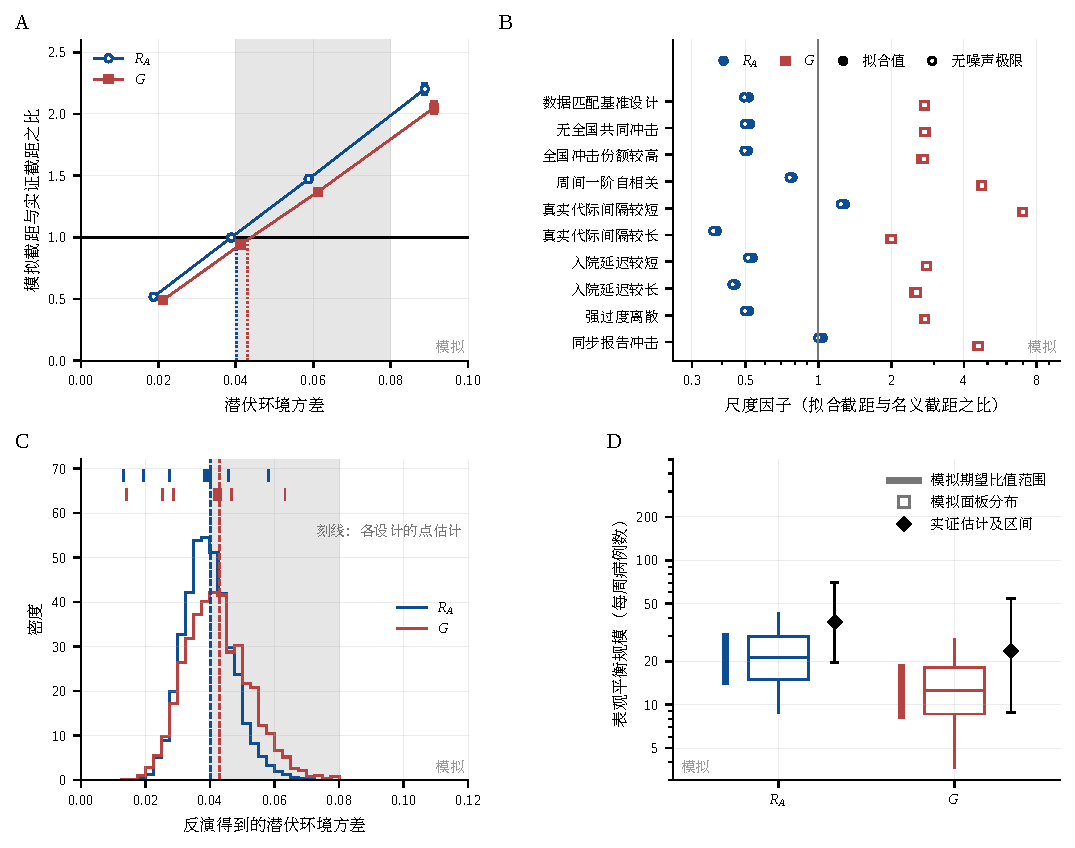
\includegraphics[width=\linewidth]{figures/fig_06_sim_inversion.pdf}
  \caption{由表观截距反演潜在环境方差的数据匹配模拟。（A）基准设计下，各潜在环境方差格点的模拟截距均值与同一统计量实证截距之比，误差线为格点均值的 95\% 蒙特卡罗区间（每格 200 个模拟面板），点线标出与实证截距的交点；灰带为 $v_R=0.04$--0.08。（B）各模拟设计在最近格点的尺度因子 $\kappa$，实心为拟合值，空心为无噪声极限。（C）基准设计下隐含环境方差的分布，合并实证截距的联合双向自助变异与校准线的蒙特卡罗误差，顶部刻线为其他设计的点估计。（D）模拟面板的表观平衡规模（箱体为四分位，须为 2.5\% 与 97.5\% 分位）、模拟期望比值范围（粗线），以及实证表观平衡规模及其双向自助 95\% 百分位区间。}
  \label{fig:inversion}
\end{figure}

$G$ 把多于一代的增长累积到一周之内，$R_A$ 则借助假定的代际间隔把周增长映射回代际尺度，因此两者的截距须经校准才能与 $v_R$ 比较。在数据匹配的模拟中，两种统计量的平均拟合截距均随 $v_R$ 线性上升（图~\ref{fig:inversion}A），各格点均值偏离拟合直线均不超过 0.60 个蒙特卡罗标准误。以 $v_R/\Rbar^2$ 的倍数表示，$R_A$ 的拟合截距对应尺度因子 $\kappa=0.516$，$G$ 为 2.729，与无噪声极限 0.493 和 2.745 接近（图~\ref{fig:inversion}B）。通用独立面板设计的无噪声极限为 0.485 和 2.698，与其 17 个情景的中位数 0.484 和 2.68 一致。数据匹配面板复现了数据的相依结构。同一日历周内周损失的组内相关系数在模拟中 $R_A$ 为 0.258、$G$ 为 0.310，数据中为 0.253 和 0.310；模拟 $R_A$ 截距中的全国周份额为 0.43，与数据的量级相同。逐项改变单一设定时，$R_A$ 的 $\kappa$ 对真实代际间隔最敏感。统计量仍按 3.6 天计算时，真实均值为 2.2 天对应 $\kappa=1.287$，为 4.3 天对应 0.380。其次是周间传播自相关（$\phi=0.5$ 时为 0.780）和作用于报告计数的同步冲击（1.041）。全国冲击份额、入院延迟与后代离散度对它影响很小（0.454--0.535；表~\ref{tab:s8}）。

把实证截距代入各自的校准线，$R_A$ 的隐含环境方差为 $v_R^{\mathrm{impl}}=0.040$（95\% CI：0.026, 0.056），$G$ 为 0.043（95\% CI：0.025, 0.064）（图~\ref{fig:inversion}A、C）。区间宽度几乎全部来自实证截距的自助变异，仅计校准误差时，$R_A$ 的区间为 0.0397--0.0406。两种统计量的尺度因子相差 5.3 倍，隐含方差之差为 $-0.003$（95\% CI：$-0.012$, 0.005），差值区间包含零。两个点估计都位于情景计算所用 0.04--0.08 区间的下缘。在潜在尺度上，按模拟器取值（$\Rbar=1.18$，$\rho=\rho_h=0.01$，$k=0.35$）由命题~\ref{prop:average} 得到的平衡规模为每代 30.3 例住院（95\% CI：21.7, 46.3）；表观值 37.4 定义在 $R_A$ 的尺度上，并不直接估计这一潜在量。

在十种设定下，$v_R^{\mathrm{impl}}$ 介于 0.013 与 0.063 之间（图~\ref{fig:inversion}C；表~\ref{tab:s8}）。真实代际间隔的影响最大，比统计量假定的 3.6 天短时得到 0.013 和 0.014，长时得到 0.058 和 0.063。两者之差的 95\% 区间在十种设定中的九种包含零；唯一的例外是以作用于报告计数的同步乘性冲击代替传播冲击，此时 $R_A$ 为 0.019，$G$ 为 0.029。

三项补充分析检验反演的假设（表~\ref{tab:s9}）。州--季节块内相对偏差的滞后一阶自相关，$R_A$ 为 $-0.095$（95\% CI：$-0.168$, $-0.019$），$G$ 为 0.123（95\% CI：0.039, 0.201）。即使周冲击相互独立，两种统计量也会因其构造而带有自相关（附录~\ref{app:random-denominator}）；独立冲击下模拟面板的均值为 $-0.074$ 和 0.114，数据分别位于第 31 和第 62 百分位。一阶系数为 0.25 时，数据位于第 3 和第 10 百分位；为 0.5 时低于全部模拟面板。季节性流感在家庭中的序列间隔估计为 3.6 天（95\% CI：2.9, 4.3）\citep{cowling2009estimation}。真实代际间隔均值为 2.9 天时，隐含方差对 $R_A$ 为 0.026，对 $G$ 为 0.027；为 4.3 天时为 0.058 和 0.063。数据的自相关在 2.9 天的模拟面板中位于第 2.5 和第 9 百分位，在 4.3 天时位于第 80 和第 92 百分位，并不支持较短的间隔。周住院数过度离散、方差均值比为 1.5 或 2.0 时，隐含方差保持在 0.039--0.045。同样设定下，$v_R=0.04$ 处模拟的 $b/a$ 对 $R_A$ 由 28.0 升至 68.0 和 81.0，对 $G$ 由 16.2 升至 40.2 和 48.4。这些设定下模拟的滞后一阶自相关普遍低于数据，数据在模拟分布中位于第 97.5 百分位或更高。数据因此更符合方差均值比小于 1.5 的过度离散。

在各统计量自身的尺度上，取 $v_R\in\{0.04,0.08\}$、$k\in\{0.2,0.5\}$ 与 $\rho_h\in\{0.0056,0.021\}$ 的八种组合，校准后的理论 $b/a$ 对 $R_A$ 为 13.9--31.1，对 $G$ 为 8.0--18.8（图~\ref{fig:inversion}D）。实证点估计 37.4 和 23.5 位于这两个范围之上，其 95\% 区间与之重叠。单个模拟面板的比值离散较大，95\% 落在 $R_A$ 的 8.8--42.7 和 $G$ 的 3.6--28.6 之间；实证值分别位于这两个分布的第 93 和第 91 百分位。
